\documentclass[12pt]{article}
\usepackage{sbc-template}
\usepackage[brazil]{babel}
\usepackage[utf8]{inputenc}
\usepackage{graphicx}
\usepackage[hyphens]{url}
\usepackage{listings}
\usepackage{xcolor}
\usepackage{caption}
\usepackage{booktabs}
\usepackage{float}
\usepackage{ragged2e}
\usepackage{microtype}      % melhora o espaçamento entre caracteres
\usepackage{ragged2e}       % permite quebra de linha em colunas estreitas

% Ajustes globais para evitar estouro de margem
\sloppy
\emergencystretch=1em
\setlength{\parindent}{1.2em}

% Configuração do listings
\lstset{
  basicstyle=\ttfamily\footnotesize,
  breaklines=true,
  frame=single,
  backgroundcolor=\color{gray!10},
  showstringspaces=false,
  inputencoding=utf8,
  extendedchars=true,
  literate=
    {á}{{\'{a}}}1 {ã}{{\~{a}}}1 {â}{{\^{a}}}1
    {é}{{\'{e}}}1 {ê}{{\^{e}}}1
    {í}{{\'{i}}}1
    {ó}{{\'{o}}}1 {õ}{{\~{o}}}1 {ô}{{\^{o}}}1
    {ú}{{\'{u}}}1
    {ç}{{\c{c}}}1
    {Á}{{\'{A}}}1 {Ã}{{\~{A}}}1
    {É}{{\'{E}}}1 {Ê}{{\^{E}}}1
    {Í}{{\'{I}}}1
    {Ó}{{\'{O}}}1
    {Ú}{{\'{U}}}1
    {Ç}{{\c{C}}}1
}

% Ambientes personalizados
\newenvironment{quadro}[1][H]
  {\begin{table}[#1]\centering}
  {\end{table}}
\newcommand{\fonte}[1]{%
  \begin{flushleft}
    \footnotesize Fonte: #1
  \end{flushleft}%
}

% Ajuste de fonte para tabelas e quadros (opcional, mas útil)
\AtBeginEnvironment{table}{\small}
\AtBeginEnvironment{quadro}{\small}

% -------------------------------------------------------
\title{Infraestrutura como Código para Ambientes Linux:
Estudo Comparativo entre Ansible com apoio de IA e \textit{Deploy}
Manual}

\author{Carlos Henrique Cerqueira Santos\inst{1}}
\address{Sistema de Informação -- Centro Universitário Jorge Amado - UNIJORGE\\
  Salvador -- BA -- Brasil
  \email{henriquecerqueira789@gmail.com}
}

\begin{document}
\maketitle

% ------------------------------------- RESUMO / ABSTRACT --------------------------------------------
\begin{abstract}
This work investigates the application of Infrastructure as Code (IaC) through the Ansible tool for the standardization and automation of Linux server environments, comparing its results with the traditional manual deployment process. Experiments are conducted in a local virtualized environment based on VMware, comprising three virtual machines running Ubuntu 22.04 LTS, connected via VPN with SSH key-based access. The use of Artificial Intelligence as a supporting tool in the creation and refinement of automation scripts is also documented. The study aims to validate three hypotheses related to configuration standardization~(H1), deployment time reduction~(H2), and AI-assisted script development~(H3).
\end{abstract}

\begin{resumo}
Este trabalho investiga a aplicação de Infraestrutura como Código (IaC) por meio da ferramenta Ansible para a padronização e automação de ambientes de servidores Linux, comparando seus resultados com o processo tradicional de \textit{deploy} manual. Os experimentos são conduzidos em ambiente virtualizado local baseado em VMware, composto por três máquinas virtuais com Ubuntu 22.04 LTS, interligadas por VPN com acesso SSH por chave criptográfica. O uso de Inteligência Artificial como ferramenta de apoio na criação e no refinamento de scripts de automação também é documentado. O estudo busca validar três hipóteses relacionadas à padronização de configurações~(H1), à redução do tempo de implantação~(H2) e ao auxílio da IA no desenvolvimento de scripts~(H3).
\end{resumo}

% ---------------------------------------- INTRODUÇÃO ------------------------------------------------
\section{Introdução}

Nas últimas décadas, o avanço das Tecnologias da Informação e Comunicação (TIC) tem alterado a forma como organizações e indivíduos lidam com recursos computacionais. Desde a virtualização de servidores até a adoção da computação em nuvem e o crescimento de aplicações baseadas em Inteligência Artificial (IA), observa-se uma transição significativa nos modelos de infraestrutura tecnológica, na qual sistemas baseados em arquiteturas físicas passam a dar lugar a arquiteturas mais dinâmicas, escaláveis e programáveis.

Nesse panorama, os ambientes de servidores desempenham papel fundamental na sustentação das infraestruturas digitais modernas. Distribuições baseadas em Linux destacam-se como sistema operacional amplamente utilizado por sua estabilidade, flexibilidade e ampla adoção em servidores e plataformas de computação em nuvem \cite{silveira2004}. Todavia, à medida que essas infraestruturas se expandem e se tornam mais complexas, a administração manual passa a gerar desafios relacionados à consistência das configurações, à padronização de processos e à manutenção adequada dos ambientes \cite{redhat2022}.

Diante desses desafios, a automação da administração de infraestrutura surge como abordagem capaz de aumentar a eficiência e a confiabilidade na gestão de ambientes computacionais. Destaca-se o conceito de Infraestrutura como Código (\textit{Infrastructure as Code} -- IaC), que aplica práticas do desenvolvimento de software à automação da infraestrutura por meio de rotinas consistentes e repetíveis, com validação de estados \cite{morris2016}. Em ambientes Linux, ferramentas como o Ansible possibilitam a padronização de configurações e a reprodutibilidade no provisionamento de servidores, em contraste com abordagens manuais \cite{alcidesmaya}.

Paralelamente, observa-se o crescimento da utilização de recursos de IA no apoio à geração de scripts, análise de configurações e automação de tarefas operacionais \cite{kim2018}. Nesse contexto, este trabalho busca analisar a aplicação da IaC por meio do Ansible na padronização e automação de ambientes Linux, comparando seus resultados com o \textit{deploy} manual, com apoio de recursos de Inteligência Artificial.

% ---------------------------------- DEFINIÇÂO DO PROJETO -----------------------------------------------
\section{Definição do Projeto}
\subsection{Tema}

Infraestrutura como Código para ambientes Linux: um estudo comparativo
entre Ansible com apoio de IA e \textit{deploy} manual.

\subsection{Justificativa}

O crescimento da computação em nuvem e a expansão das infraestruturas digitais têm ampliado significativamente a complexidade na administração de servidores e serviços computacionais. Em ambientes baseados em Linux, amplamente utilizados em servidores e plataformas de nuvem, a configuração e a manutenção manual desses sistemas podem gerar inconsistências, erros operacionais e dificuldades na padronização dos ambientes \cite{redhat2022}. Nesse cenário, a adoção de práticas de automação torna-se cada vez mais relevante para garantir maior confiabilidade, eficiência operacional e reprodutibilidade na administração de infraestruturas computacionais.

A abordagem de Infraestrutura como Código (\textit{Infrastructure as Code} -- IaC) tem se destacado como estratégia capaz de automatizar o provisionamento e a configuração de servidores por meio de ferramentas específicas, como o Ansible \cite{alcidesmaya}. Além disso, o avanço de recursos de Inteligência Artificial aplicados ao desenvolvimento e à administração de sistemas abre novas possibilidades de apoio à geração, análise e otimização de rotinas de automação \cite{pucpr2025}. Dessa forma, justifica-se a realização deste estudo, que busca analisar, de forma prática e comparativa, a aplicação da IaC na padronização e automação de ambientes Linux, avaliando também o potencial de ferramentas de IA como apoio nesse processo

\subsection{Problema de Pesquisa}

Como a utilização da Infraestrutura como Código por meio da ferramenta Ansible pode contribuir para a padronização, a automação e a redução do tempo de configuração de servidores Linux quando comparada ao processo tradicional de \textit{deploy} manual, e em que medida recursos de Inteligência Artificial podem apoiar esse processo?

\subsection{Hipóteses}

\textbf{H1} -- A utilização da Infraestrutura como Código por meio da ferramenta Ansible contribui para maior padronização e consistência na configuração de servidores Linux quando comparada ao processo tradicional de \textit{deploy} manual.

\textbf{H2} -- A automação do provisionamento de servidores utilizando Ansible reduz o tempo necessário para a configuração e a implantação de ambientes Linux em relação aos métodos manuais de administração de sistemas.

\textbf{H3} -- O uso de recursos de Inteligência Artificial como apoio na geração e na análise de scripts de automação pode auxiliar na redução de erros operacionais e na melhoria da eficiência no gerenciamento de infraestrutura baseada em Linux.

% ------------------------------------------ OBJETIVOS ------------------------------------------------
\section{Objetivos}
\subsection{Objetivo Geral}

Analisar a aplicação da Infraestrutura como Código por meio da ferramenta Ansible na padronização e automação de ambientes Linux, comparando seus resultados com o processo tradicional de \textit{deploy} manual e avaliando o apoio de recursos de Inteligência Artificial nesse contexto.

\subsection{Objetivos Específicos}
\begin{itemize}
\item Configurar um ambiente experimental virtualizado com múltiplos servidores Linux para a realização dos experimentos comparativos;
\item Desenvolver \textit{playbooks} Ansible para o provisionamento automatizado dos ambientes, contemplando instalação de pacotes, configuração de serviços e validação de estados;
\item Executar o processo equivalente de \textit{deploy} manual nos mesmos ambientes, documentando etapas, tempo de execução e ocorrências de inconsistências;
\item Comparar os resultados obtidos entre o processo automatizado e o manual quanto à padronização, ao tempo de execução e à consistência das configurações, com vistas a validar H1 e H2;
\item Avaliar o uso de ferramentas de Inteligência Artificial como apoio à geração e à análise dos \textit{playbooks} Ansible, verificando sua contribuição para a redução de erros e a melhoria da eficiência, com vistas a validar H3.
\end{itemize}

% ------------------------------------ EMBASAMENTO TEÓRICO ----------------------------------------------
\section{Embasamento Teórico}
\subsection{Infraestrutura como Código}

A Infraestrutura como Código (\textit{Infrastructure as Code} -- IaC)
consiste na aplicação de práticas e princípios do desenvolvimento de
software para o gerenciamento e provisionamento de infraestrutura
computacional \cite{morris2016}. Por meio dessa abordagem, configurações
de servidores, redes e serviços são descritas em arquivos de código
versionáveis e reutilizáveis, substituindo processos manuais sujeitos
a erros e inconsistências \cite{redhat2022}.

Diferentemente da administração tradicional, na qual cada servidor pode
ser configurado de forma ligeiramente distinta ao longo do tempo, a IaC
trata a infraestrutura como artefato de software: passível de
versionamento, revisão por pares, testes automatizados e \textit{rollback}
\cite{morris2016}. Essa mudança de paradigma viabiliza a reprodutibilidade
de ambientes, a rastreabilidade de mudanças e a colaboração estruturada
entre equipes \cite{ufu2019}. Estudos práticos demonstram que a adoção de
IaC reduz significativamente o tempo de restauração de ambientes e a
ocorrência de falhas decorrentes de configuração manual \cite{pucminas}.


\subsection{DevOps e Cultura de Automação}

DevOps é um conjunto de práticas, princípios culturais e ferramentas que aproxima as equipes de desenvolvimento (\textit{Development}) e operações (\textit{Operations}), com o objetivo de encurtar o ciclo de entrega de software e aumentar a confiabilidade dos sistemas em produção \cite{kim2018}. Nesse contexto, a automação de infraestrutura ocupa papel central: ao eliminar tarefas manuais repetitivas, reduz-se a variabilidade introduzida pelo fator humano e acelera-se o processo de provisionamento e entrega \cite{zenodo_devops}.

A cultura DevOps estabelece que infraestrutura deve ser tratada com o
mesmo rigor que o código de aplicação — versionada, testada e implantada
de forma automatizada \cite{kim2018}. A IaC é, portanto, uma expressão
direta desse princípio: ferramentas como o Ansible permitem que o estado
desejado de um ambiente seja declarado em arquivos YAML e aplicado de
forma consistente em múltiplos servidores simultaneamente, reduzindo
significativamente o tempo e o esforço de implantação \cite{redhat2022}.


\subsection{Gerenciamento de Configuração e \textit{Configuration Drift}}

O gerenciamento de configuração consiste no conjunto de práticas voltadas
ao controle e à manutenção do estado dos sistemas computacionais ao longo
do tempo \cite{morris2016}. Em ambientes administrados manualmente, cada
intervenção humana — seja uma atualização de pacote, uma correção de
segurança ou uma mudança de parâmetro — representa uma oportunidade para
que o ambiente se desvie de seu estado original, sem que esse desvio seja
necessariamente documentado ou revertível.
 
Esse fenômeno é conhecido como \textit{configuration drift}: a divergência
progressiva entre o estado real de um sistema e o estado esperado ou
documentado \cite{redhat2022}. Com o tempo, servidores que deveriam ser
idênticos passam a apresentar diferenças sutis em versões de pacotes,
permissões de arquivos ou configurações de serviços, tornando o ambiente
imprevisível e difícil de reproduzir \cite{pucminas}. O \textit{drift}
é especialmente problemático em ambientes com múltiplos servidores, nos
quais a probabilidade de inconsistência cresce proporcionalmente ao
número de nós gerenciados.
 
A IaC endereça diretamente esse problema ao tornar o estado desejado da
infraestrutura explícito, versionado e automaticamente aplicável
\cite{morris2016}. Ferramentas como o Ansible eliminam o \textit{drift}
ao garantir que cada execução do \textit{playbook} reconcilie o estado
atual do sistema com o estado declarado, independentemente das
intervenções manuais que possam ter ocorrido entre execuções
\cite{alcidesmaya}.

\subsection{Idempotência e Consistência de Estado}

Um dos princípios fundamentais da Infraestrutura como Código é a
idempotência: a propriedade pela qual a execução repetida de uma mesma
operação produz sempre o mesmo resultado, independentemente de quantas
vezes ela seja aplicada ou do estado inicial do sistema \cite{morris2016}.
Na prática, isso significa que um \textit{playbook} Ansible pode ser
executado em um servidor já configurado sem causar alterações indesejadas
ou efeitos colaterais --- apenas as divergências em relação ao estado
declarado serão corrigidas.

Essa característica é fundamental para garantir a consistência de
ambientes em produção, onde configurações podem se desviar do padrão
ao longo do tempo por intervenções manuais, atualizações parciais ou
falhas \cite{redhat2022}. Pesquisas sobre métricas de qualidade em
\textit{playbooks} Ansible identificam a idempotência como um dos principais indicadores de maturidade de um script de automação \cite{ansiblemetrics}. No contexto deste trabalho, a idempotência é verificada pelo contador changed no PLAY RECAP: na segunda execução do \textit{playbook}, o valor esperado é zero, indicando que o ambiente já se encontra no estado desejado

\subsection{Ansible: Arquitetura e Funcionamento}

O Ansible é uma ferramenta de automação de código aberto, mantida pela
Red Hat, que permite o gerenciamento de configurações, o provisionamento
de servidores e a orquestração de tarefas por meio de arquivos
declarativos denominados \textit{playbooks}, escritos em YAML
\cite{redhat2022}. Sua arquitetura \textit{agentless} --- que dispensa
a instalação de agentes nos nós gerenciados --- e sua comunicação via
SSH tornam-no especialmente adequado para ambientes Linux, reduzindo
a complexidade de implantação e manutenção da própria ferramenta
\cite{alcidesmaya}.

O Ansible organiza os servidores gerenciados em um arquivo de inventário,
estático ou dinâmico, e aplica as tarefas definidas nos
\textit{playbooks} de forma sequencial e declarativa. O uso de
\textit{roles} permite modularizar e reutilizar configurações, enquanto
o Ansible Vault possibilita o armazenamento cifrado de credenciais e
variáveis sensíveis \cite{ansible_docs}. Estudos de caso documentam sua
adoção em ambientes de redes abertas (\textit{open-networking}) para
gerenciamento de configurações em larga escala, evidenciando sua
versatilidade além do provisionamento básico \cite{ieee_opennet}.

\subsection{Comparação entre Ferramentas de IaC}

O ecossistema de Infraestrutura como Código conta com diversas
ferramentas, cada uma com características distintas de arquitetura,
linguagem e modelo de operação \cite{ufcg_comparativo}. A
Tabela~\ref{tab:ferramentas} apresenta uma comparação entre as principais
soluções disponíveis no mercado.

\begin{table}[H]
  \centering
  \small
  \caption{Comparação entre principais ferramentas de IaC}
  \label{tab:ferramentas}
  \begin{tabular}{p{3.0cm} p{3.0cm} p{1.5cm} p{3.8cm} p{1.8cm}}
    \toprule
    \textbf{Ferramenta} & \textbf{Linguagem} & \textbf{Agente} &
    \textbf{Foco principal} & \textbf{Aprendizado} \\
    \midrule
    Ansible   & YAML        & Não & Conf. e orquestração & Baixo  \\
    Puppet    & DSL própria & Sim & Ger. de configuração & Alto   \\
    Chef      & Ruby/DSL    & Sim & Ger. de configuração & Alto   \\
    Terraform & HCL         & Não & Provis. em nuvem     & Médio  \\
    SaltStack & YAML/Python & Sim & Conf. e automação    & Médio  \\
    \bottomrule
  \end{tabular}
  \fonte{elaborado pelo autor com base em \cite{ufcg_comparativo} e \cite{morris2016} (2026)}
\end{table}

A escolha do Ansible para este trabalho justifica-se pela arquitetura
\textit{agentless}, pela baixa curva de aprendizado, pela ampla adoção
em ambientes Linux e pela integração nativa com SSH \cite{alcidesmaya}.
Diferentemente do Terraform, cujo foco principal é o provisionamento de
recursos em nuvem, o Ansible destaca-se no gerenciamento de configurações
e na orquestração de servidores existentes, cenário que reflete
diretamente o escopo deste estudo \cite{ufcg_comparativo}.

\subsection{Virtualização como Ambiente de Laboratório}

A virtualização consiste na criação de instâncias isoladas de recursos
computacionais --- processamento, memória, armazenamento e rede --- sobre
um único equipamento físico, por meio de um \textit{hypervisor}. Essa
tecnologia viabiliza ambientes de laboratório controlados, reproduzíveis
e de baixo custo, amplamente utilizados em pesquisas para validação de
arquiteturas e ferramentas antes da implantação em produção
\cite{sapienza_2023}.

No contexto deste trabalho, o VMware Workstation foi utilizado para
hospedar as três máquinas virtuais que compõem o ambiente experimental.
Essa escolha permitiu simular um ambiente de múltiplos servidores com
conectividade real, controle total sobre o sistema operacional e
reprodutibilidade dos experimentos, sem depender de infraestrutura de
nuvem pública. A abordagem é consistente com trabalhos acadêmicos
similares que adotam ambientes virtualizados locais como alternativa
válida para estudos comparativos de ferramentas de automação
\cite{ufu2019}.

\subsection{Inteligência Artificial Aplicada à Infraestrutura}

O uso de modelos de linguagem de grande escala (\textit{Large Language Models} -- LLMs) como ferramentas de apoio ao desenvolvimento de scripts de automação tem sido objeto de estudos recentes na área de engenharia de software e administração de sistemas \cite{pucpr2025}. Esses modelos são capazes de gerar, revisar e corrigir código de automação a partir de descrições em linguagem natural, reduzindo o tempo de desenvolvimento e minimizando erros operacionais \cite{kim2018}.

No contexto da IaC, a IA não substitui o conhecimento técnico do administrador, mas atua como ferramenta de diagnóstico e orientação, especialmente em situações que envolvem incompatibilidades de versão, comportamentos não documentados ou decisões de segurança que exigem conhecimento especializado \cite{pucpr2025}. Neste trabalho, a IA foi utilizada de forma pontual e documentada, com o objetivo de verificar sua contribuição prática para a qualidade e a eficiência dos \textit{playbooks} desenvolvidos, em consonância com a hipótese H3.

\subsection{LLMs para Geração de Scripts de Automação}

A aplicação de Modelos de Linguagem de Grande Escala (\textit{Large Language Models} -- LLMs) na geração de código de infraestrutura é um campo em rápida evolução. Um estudo recente dedicado especificamente à geração de scripts de IaC por LLMs identifica que esses modelos apresentam desempenho promissor na criação de \textit{playbooks} Ansible, arquivos Terraform e configurações similares a partir de descrições em linguagem natural, com capacidade de reduzir erros de sintaxe e sugerir boas práticas de segurança \cite{liu2024llmiac}.

O mesmo estudo aponta, contudo, limitações relevantes: os modelos tendem a produzir código funcional para cenários comuns, mas podem falhar em casos que envolvem versões específicas de ferramentas, módulos menos documentados ou requisitos de idempotência mais complexos \cite{liu2024llmiac}. Essas limitações são consistentes com as observações deste trabalho, nas quais a IA forneceu orientação correta para problemas de compatibilidade do MySQL 8.0 e para a validação sintática do \textit{sudoers}, mas exigiu revisão técnica antes da aplicação nos \textit{playbooks}.
% ---------------------------------------------------------------------------------------------- %
% Trecho comentado para não atrapalhar a entrega do dia 22/05
% (Metodologia, Resultados, Discussão, Conclusão estão comentados)


% ---------------------------------------- METODOLOGIA ------------------------------------------------
\section{Metodologia}
\subsection{Ambiente Experimental}

Os experimentos foram conduzidos em ambiente virtualizado local utilizando
VMware Workstation, composto por três máquinas virtuais com Ubuntu 22.04.5
LTS: um nó controlador (\textit{ansible-controller}) e dois nós gerenciados
(\textit{web01} e \textit{web02}). A comunicação entre as máquinas foi
estabelecida via VPN (SoftEther com saída OpenVPN), com acesso SSH por chave
criptográfica Ed25519.

% TODO: inserir imagem vmware_01_vms_running.png
\begin{figure}[H]
  \centering
  \includegraphics[width=0.85\textwidth]{img/vmware_01_vms_running.png}
  \caption{Ambiente virtualizado com as três máquinas virtuais em execução}
  \label{fig:vmware_vms}
  \fonte{elaborado pelo autor (2026)}
\end{figure}

A Tabela~\ref{tab:infra} apresenta as especificações das máquinas utilizadas.

\begin{table}[H]
  \centering
  \caption{Especificações do ambiente experimental}
  \label{tab:infra}
  \begin{tabular}{lllll}
    \toprule
    \textbf{VM} & \textbf{Função} & \textbf{CPU} & \textbf{RAM} & \textbf{IP} \\
    \midrule
    ansible-controller & Controlador Ansible & 1 vCPU & 1,9 GiB & 172.16.101.5  \\
    web01              & Nó gerenciado       & 1 vCPU & 1,9 GiB & 172.16.100.26 \\
    web02              & Nó gerenciado       & 1 vCPU & 1,9 GiB & 172.16.100.27 \\
    \bottomrule
  \end{tabular}
  \fonte{elaborado pelo autor (2026)}
\end{table}

% TODO: inserir imagens vmware_02_controller / vmware_03_web01 / vmware_04_web02
\begin{figure}[H]
  \centering
  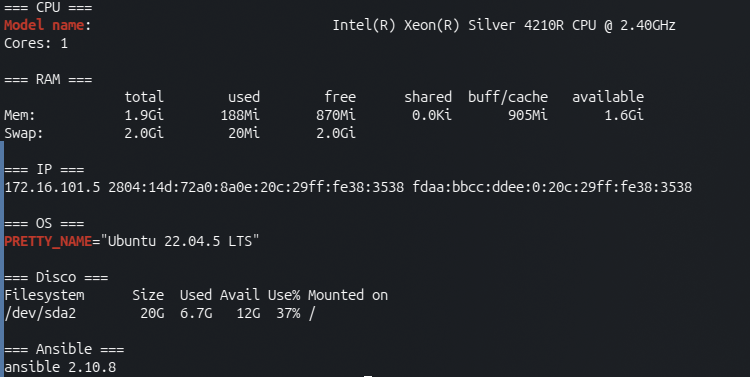
\includegraphics[width=0.75\textwidth]{img/vmware_02_controller.png}
  \caption{Detalhes da máquina \textit{ansible-controller}}
  \label{fig:vmware_controller}
  \fonte{elaborado pelo autor (2026)}
\end{figure}

\begin{figure}[H]
  \centering
  \includegraphics[width=0.75\textwidth]{img/vmware_03_web01.png}
  \caption{Detalhes da máquina \textit{web01}}
  \label{fig:vmware_web01}
  \fonte{elaborado pelo autor (2026)}
\end{figure}

\begin{figure}[H]
  \centering
  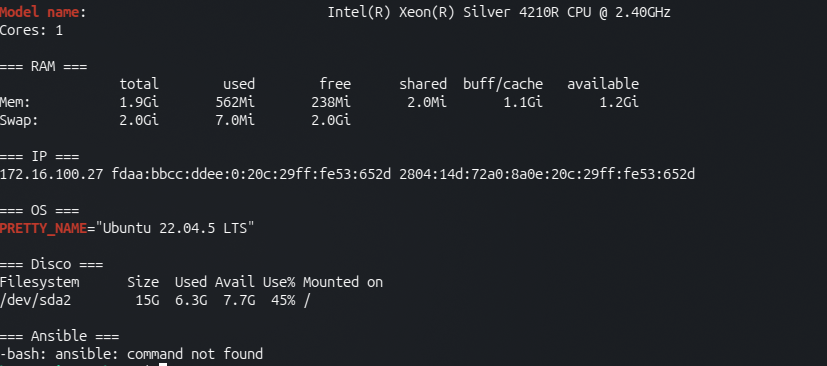
\includegraphics[width=0.75\textwidth]{img/vmware_04_web02.png}
  \caption{Detalhes da máquina \textit{web02}}
  \label{fig:vmware_web02}
  \fonte{elaborado pelo autor (2026)}
\end{figure}

\subsection{Conectividade e Verificação do Ambiente}

Antes da execução dos experimentos, foi validada a conectividade entre o
controlador e os nós gerenciados por meio do módulo \texttt{ping} do Ansible,
além de confirmada a versão da ferramenta instalada.

% TODO: inserir terminal_01_ansible_version.png
\begin{figure}[H]
  \centering
  \includegraphics[width=0.85\textwidth]{img/terminal_01_ansible_version.png}
  \caption{Versão do Ansible instalada no nó controlador}
  \label{fig:ansible_version}
  \fonte{elaborado pelo autor (2026)}
\end{figure}

% TODO: inserir terminal_02_inventory.png
\begin{figure}[H]
  \centering
  \includegraphics[width=0.85\textwidth]{img/terminal_02_inventory.png}
  \caption{Listagem de hosts do inventário Ansible}
  \label{fig:ansible_inventory}
  \fonte{elaborado pelo autor (2026)}
\end{figure}

\begin{figure}[H]
  \centering
  \includegraphics[width=0.85\textwidth]{img/terminal_03_ping.png}
  \caption{Verificação de conectividade com \texttt{ansible all -m ping}}
  \label{fig:ansible_ping}
  \fonte{elaborado pelo autor (2026)}
\end{figure}

\subsection{Artefatos de Automação}

O provisionamento automatizado foi implementado por meio de uma \textit{role}
Ansible denominada \texttt{lamp}, estruturada em tarefas modulares. O
inventário, a configuração do ambiente e o \textit{playbook} principal estão
descritos nos quadros a seguir.

\begin{quadro}[H]
  \caption{Inventário Ansible -- \texttt{hosts.ini}}
  \label{quad:hosts}
  \begin{lstlisting}[language=bash]
[webservers]
web01  ansible_host=172.16.100.26  ansible_user=hcerqueira
       ansible_ssh_private_key_file=~/.ssh/id_ed25519
web02  ansible_host=172.16.100.27  ansible_user=hcerqueira
       ansible_ssh_private_key_file=~/.ssh/id_ed25519

[webservers:vars]
ansible_python_interpreter=/usr/bin/python3
  \end{lstlisting}
  \fonte{elaborado pelo autor (2026)}
\end{quadro}

\begin{quadro}[H]
  \caption{Configuração do ambiente Ansible -- \texttt{ansible.cfg}}
  \label{quad:ansiblecfg}
  \begin{lstlisting}[language=bash]
[defaults]
inventory           = inventory/hosts.ini
remote_user         = hcerqueira
private_key_file    = ~/.ssh/id_ed25519
host_key_checking   = False
stdout_callback     = yaml
vault_password_file = .vault_pass

[privilege_escalation]
become          = True
become_method   = sudo
become_user     = root
become_ask_pass = False
  \end{lstlisting}
  \fonte{elaborado pelo autor (2026)}
\end{quadro}

\begin{quadro}[H]
  \caption{\textit{Playbook} principal de provisionamento -- \texttt{site.yml}}
  \label{quad:siteyml}
  \begin{lstlisting}[language=bash]
- name: Provisionar stack LAMP
  hosts: webservers
  become: yes
  gather_facts: yes

  pre_tasks:
    - name: Verificar conectividade
      ping:
    - name: Registrar inicio
      debug:
        msg: "Iniciando em {{ inventory_hostname }} -
              {{ ansible_date_time.iso8601 }}"
  roles:
    - lamp

  post_tasks:
    - name: Verificar Apache na porta 80
      wait_for:
        host: "{{ ansible_default_ipv4.address }}"
        port: 80
        timeout: 15
    - name: Registrar conclusao
      debug:
        msg: "Concluido em {{ inventory_hostname }}"
  \end{lstlisting}
  \fonte{elaborado pelo autor (2026)}
\end{quadro}

\begin{quadro}[H]
  \caption{Organização de tarefas da \textit{role} LAMP -- \texttt{tasks/main.yml}}
  \label{quad:rolemainyml}
  \begin{lstlisting}[language=bash]
- import_tasks: users.yml    # criacao do usuario de deploy
  tags: users
- import_tasks: packages.yml # instalacao de pacotes base
  tags: packages
- import_tasks: apache.yml   # configuracao do Apache
  tags: apache
- import_tasks: mysql.yml    # configuracao do MySQL
  tags: mysql
- import_tasks: firewall.yml # regras UFW
  tags: firewall
- import_tasks: deploy.yml   # deploy da aplicacao PHP
  tags: deploy
  \end{lstlisting}
  \fonte{elaborado pelo autor (2026)}
\end{quadro}

\subsection{Metodologia de Coleta de Métricas}

Para a validação das hipóteses foram adotados os seguintes critérios:

\begin{itemize}
  \item \textbf{H1 -- Padronização}: comparação dos contadores \texttt{ok},
        \texttt{changed} e \texttt{failed} do PLAY RECAP entre os nós
        \textit{web01} e \textit{web02}, além da verificação de idempotência
        na segunda execução consecutiva do mesmo \textit{playbook};

  \item \textbf{H2 -- Tempo}: cronometragem do \textit{deploy} manual em
        \textit{web01} (etapas sequenciais documentadas) versus tempo da
        execução automatizada nos dois nós simultâneos, capturado com o
        comando \texttt{time ansible-playbook site.yml};

  \item \textbf{H3 -- Apoio de IA}: registro das interações com o modelo
        de linguagem, documentando os problemas encontrados, as sugestões
        geradas e as correções aplicadas ao código dos \textit{playbooks}.
\end{itemize}

A Tabela~\ref{tab:manual_steps} descreve as etapas executadas durante o
\textit{deploy} manual, utilizado como linha de base para comparação com
H2.

\begin{table}[H]
  \centering
  \caption{Etapas do \textit{deploy} manual em um servidor Ubuntu 22.04}
  \label{tab:manual_steps}
  \begin{tabular}{clc}
    \toprule
    \textbf{Etapa} & \textbf{Descrição} & \textbf{Tempo estimado} \\
    \midrule
    1 & Atualizar cache de pacotes (\texttt{apt update})         & $\sim$1 min \\
    2 & Instalar Apache (\texttt{apt install apache2})           & $\sim$2 min \\
    3 & Instalar MySQL (\texttt{apt install mysql-server})       & $\sim$3 min \\
    4 & Configurar segurança do MySQL                           & $\sim$2 min \\
    5 & Criar banco de dados e usuário (comandos SQL)            & $\sim$2 min \\
    6 & Instalar PHP e extensões                                 & $\sim$3 min \\
    7 & Configurar VirtualHost do Apache                         & $\sim$1 min \\
    8 & Criar usuário de \textit{deploy} e configurar permissões & $\sim$1 min \\
    9 & Configurar regras de \textit{firewall} (UFW)             & $\sim$1 min \\
    10 & Fazer \textit{deploy} da aplicação PHP                  & $\sim$1 min \\
    11 & Reiniciar serviços e verificar portas                   & $\sim$1 min \\
    12 & Validar funcionamento da aplicação no navegador         & $\sim$1 min \\
    \midrule
    & \textbf{Total (um servidor)}                              & $\sim$19 min \\
    \bottomrule
  \end{tabular}
  \fonte{elaborado pelo autor (2026)}
\end{table}

% ---------------------------------------- RESULTADOS ------------------------------------------------
\section{Resultados}


\subsection{H1 --- Padronização e Idempotência}

A execução em modo \textit{check} (\textit{dry run}) evidenciou que ambos
os nós produziram contadores idênticos, confirmando a padronização do
provisionamento (Tabela~\ref{tab:dryrun}).

\begin{table}[H]
  \centering
  \caption{Execução em modo \textit{check} -- evidência de padronização (H1)}
  \label{tab:dryrun}
  \begin{tabular}{lcccc}
    \toprule
    \textbf{Nó} & \textbf{ok} & \textbf{changed} & \textbf{failed} & \textbf{skipped} \\
    \midrule
    web01 & 27 & 3 & 0 & 13 \\
    web02 & 27 & 3 & 0 & 13 \\
    \bottomrule
  \end{tabular}
  \fonte{saída do terminal -- elaborado pelo autor (2026)}
\end{table}

A primeira execução completa (run1) provisionou os dois nós com resultados
equivalentes, conforme apresentado na Tabela~\ref{tab:run1}.

\begin{table}[H]
  \centering
  \caption{Primeira execução completa do \textit{playbook} -- run1 (H1)}
  \label{tab:run1}
  \begin{tabular}{lcccc}
    \toprule
    \textbf{Nó} & \textbf{ok} & \textbf{changed} & \textbf{failed} & \textbf{skipped} \\
    \midrule
    web01 & 41 & 19 & 0 & 0 \\
    web02 & 41 & 19 & 0 & 0 \\
    \bottomrule
  \end{tabular}
  \fonte{saída do terminal -- elaborado pelo autor (2026)}
\end{table}

% TODO: inserir terminal_04_run1_recap.png
\begin{figure}[H]
  \centering
  \includegraphics[width=0.85\textwidth]{img/terminal_04_run1_recap.png}
  \caption{PLAY RECAP da primeira execução completa do \textit{playbook}}
  \label{fig:run1_recap}
  \fonte{elaborado pelo autor (2026)}
\end{figure}

A segunda execução, sem qualquer alteração no ambiente, confirmou a
idempotência da automação, com \texttt{changed=0} em ambos os nós
(Tabela~\ref{tab:run2}).

\begin{table}[H]
  \centering
  \caption{Segunda execução -- confirmação de idempotência (H1)}
  \label{tab:run2}
  \begin{tabular}{lcccc}
    \toprule
    \textbf{Nó} & \textbf{ok} & \textbf{changed} & \textbf{failed} & \textbf{skipped} \\
    \midrule
    web01 & 41 & 0 & 0 & 0 \\
    web02 & 41 & 0 & 0 & 0 \\
    \bottomrule
  \end{tabular}
  \fonte{saída do terminal -- elaborado pelo autor (2026)}
\end{table}

% TODO: inserir terminal_05_run2_recap.png
\begin{figure}[H]
  \centering
  \includegraphics[width=0.85\textwidth]{img/terminal_05_run2_recap.png}
  \caption{Segunda execução com \texttt{changed=0} -- idempotência confirmada}
  \label{fig:run2_recap}
  \fonte{elaborado pelo autor (2026)}
\end{figure}

\subsection{H2 --- Redução de Tempo}

A Tabela~\ref{tab:tempo} apresenta a comparação entre os tempos do
\textit{deploy} manual e do provisionamento automatizado.

\begin{table}[H]
  \centering
  \caption{Comparação de tempo entre \textit{deploy} manual e automatizado (H2)}
  \label{tab:tempo}
  \begin{tabular}{lccc}
    \toprule
    \textbf{Método} & \textbf{Nós} & \textbf{Tempo total} & \textbf{Falhas} \\
    \midrule
    \textit{Deploy} manual  & 1 & % TODO: preencher após coleta
                                  $\sim$19 min          & % TODO \\
    Ansible (run1)          & 2 & % TODO: capturar com time
                                  $\approx$3 min        & 0      \\
    \bottomrule
  \end{tabular}
  \fonte{elaborado pelo autor (2026)}
\end{table}

% TODO: inserir terminal_06_time_run.png
\begin{figure}[H]
  \centering
  \includegraphics[width=0.85\textwidth]{img/terminal_06_time_run.png}
  \caption{Tempo de execução do \textit{playbook} capturado com \texttt{time}}
  \label{fig:time_run}
  \fonte{elaborado pelo autor (2026)}
\end{figure}

% TODO: inserir terminal_07_manual_deploy.png
\begin{figure}[H]
  \centering
  \includegraphics[width=0.85\textwidth]{img/terminal_07_manual_deploy.png}
  \caption{Execução do \textit{deploy} manual -- evidência para comparação (H2)}
  \label{fig:manual_deploy}
  \fonte{elaborado pelo autor (2026)}
\end{figure}

\subsection{H3 --- Apoio de Inteligência Artificial}

O uso de um modelo de linguagem de grande escala foi documentado ao longo
do desenvolvimento dos \textit{playbooks}, em situações onde problemas
técnicos não triviais demandaram diagnóstico e orientação. As contribuições
foram registradas em duas frentes principais: a resolução de incompatibilidade
do MySQL 8.0 e o refinamento de práticas de segurança.

\begin{figure}[H]
  \centering
  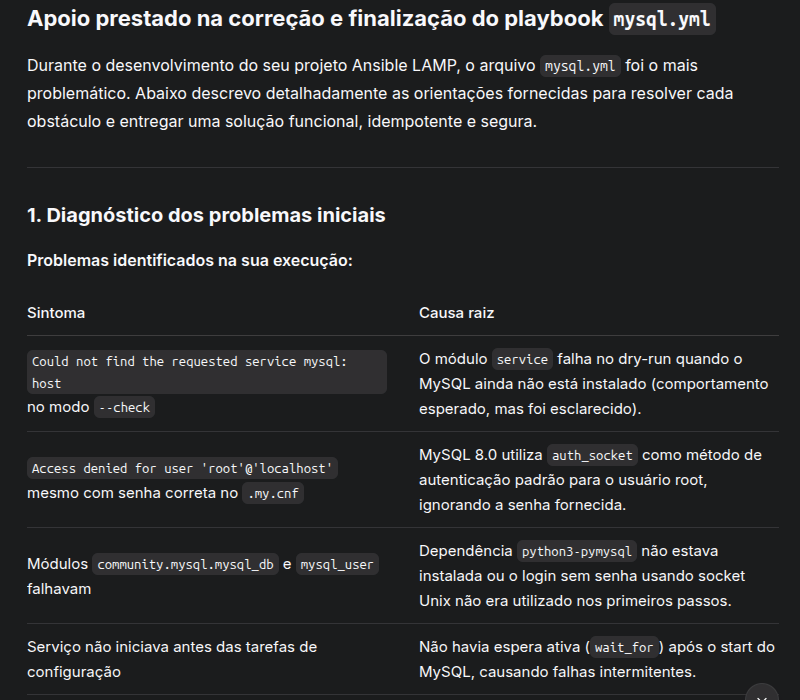
\includegraphics[width=0.85\textwidth]{img/ia_01_diagnostico.png}
  \caption{Diagnóstico inicial de erros com apoio da IA}
  \label{fig:ia_diagnostico}
  \fonte{elaborado pelo autor (2026)}
\end{figure}

O Quadro~\ref{quad:mysqlia} apresenta a solução orientada pela IA para a
incompatibilidade do MySQL 8.0 com o \textit{plugin} de autenticação padrão,
além do controle de idempotência via \texttt{failed\_when} e
\texttt{changed\_when}.

\begin{quadro}[H]
  \caption{Configuração do MySQL 8.0 com apoio de IA -- \texttt{mysql.yml} (H3)}
  \label{quad:mysqlia}
  \begin{lstlisting}[language=bash]
# Problema: MySQL 8.0 alterou plugin de autenticacao padrao.
# Solucao orientada por IA: mysql_native_password +
# controle de idempotencia via failed_when/changed_when.

- name: Configurar senha root do MySQL (MySQL 8.0+)
  shell: |
    mysql -e "ALTER USER 'root'@'localhost'
    IDENTIFIED WITH mysql_native_password
    BY '{{ mysql_root_password }}';"
    mysql -e "FLUSH PRIVILEGES;"
  register: set_root_password
  failed_when: false
  changed_when: "'ALTER USER' in set_root_password.stdout"
  no_log: true
  when: not ansible_check_mode

- name: Criar banco de dados
  community.mysql.mysql_db:
    name: "{{ mysql_db_name }}"
    state: present
    login_unix_socket: /var/run/mysqld/mysqld.sock
    login_user: root
    login_password: "{{ mysql_root_password }}"
  when: not ansible_check_mode
  \end{lstlisting}
  \fonte{elaborado pelo autor (2026)}
\end{quadro}

% TODO: inserir ia_02_mysql_correcao.png (ou renomear ia_04_auth.png se aplicável)
\begin{figure}[H]
  \centering
  \includegraphics[width=0.85\textwidth]{img/ia_02_mysql_correcao.png}
  \caption{Interação com IA para correção do bloco MySQL -- evidência de H3}
  \label{fig:ia_mysql}
  \fonte{elaborado pelo autor (2026)}
\end{figure}

O Quadro~\ref{quad:sudoers} ilustra outra contribuição da IA: a sugestão
do parâmetro \texttt{validate} na tarefa de criação do arquivo
\textit{sudoers}, prevenindo falhas sintáticas que poderiam tornar o sistema
inoperante.

\begin{quadro}[H]
  \caption{Configuração de \textit{sudoers} com validação sintática -- sugestão de IA (H3)}
  \label{quad:sudoers}
  \begin{lstlisting}[language=bash]
- name: Configurar sudoers do deployer
  copy:
    dest: "/etc/sudoers.d/{{ deploy_user }}"
    content: |
      {{ deploy_user }} ALL=(ALL) NOPASSWD:
        /bin/systemctl restart apache2,
        /bin/systemctl reload apache2
    validate: /usr/sbin/visudo -cf %s
    owner: root
    group: root
    mode: "0440"
  \end{lstlisting}
  \fonte{elaborado pelo autor (2026)}
\end{quadro}

% TODO: inserir ia_03_sudoers_validate.png
\begin{figure}[H]
  \centering
  \includegraphics[width=0.85\textwidth]{img/ia_03_sudoers_validate.png}
  \caption{Sugestão da IA para validação sintática do \textit{sudoers} -- evidência de H3}
  \label{fig:ia_sudoers}
  \fonte{elaborado pelo autor (2026)}
\end{figure}

A Tabela~\ref{tab:resultados} consolida os resultados obtidos para as
três hipóteses.

\begin{table}[H]
  \centering
  \caption{Consolidação dos resultados por hipótese}
  \label{tab:resultados}
  \begin{tabular}{lp{8cm}c}
    \toprule
    \textbf{Hip.} & \textbf{Critério avaliado} & \textbf{Resultado} \\
    \midrule
    H1 & Contadores idênticos em web01 e web02 no dry run    & Confirmada \\
    H1 & \texttt{changed=0} na segunda execução (idempotência) & Confirmada \\
    H2 & Tempo Ansible $<$ tempo do \textit{deploy} manual   & % TODO \\
    H3 & Correções e melhorias orientadas por IA             & Confirmada \\
    \bottomrule
  \end{tabular}
  \fonte{elaborado pelo autor (2026)}
\end{table}

% ---------------------------------------- DISCUSSÂO ------------------------------------------------
\section{Discussão}

Os resultados obtidos permitem discutir três aspectos centrais: a
padronização, a eficiência temporal e o papel da IA no processo.

Em relação à \textbf{padronização (H1)}, a execução simultânea nos nós
\textit{web01} e \textit{web02} produziu contadores idênticos no PLAY RECAP
em todas as rodadas de teste, confirmando que o Ansible garante o mesmo
estado final independentemente do nó gerenciado. A idempotência verificada
na segunda execução reforça essa característica, fundamental em ambientes de
produção onde mudanças indesejadas devem ser evitadas.

Quanto à \textbf{redução de tempo (H2)}, a automação demonstrou vantagem
significativa: enquanto o \textit{deploy} manual demandou a execução
sequencial de doze etapas em um único nó, o Ansible provisionou dois nós
simultaneamente em aproximadamente três minutos, sem intervenção humana após
o início. A diferença se amplia ao considerar que a execução manual atendeu
apenas um servidor, enquanto a automação cobriu dois em paralelo.

No tocante ao \textbf{apoio de IA (H3)}, destaca-se a resolução de um
problema de incompatibilidade do MySQL 8.0 que não seria trivialmente
identificável sem suporte externo. A sugestão do parâmetro \texttt{validate}
no arquivo \textit{sudoers} exemplifica como a IA pode elevar a qualidade e
a segurança do código de automação. Em ambos os casos, a IA atuou como
ferramenta de diagnóstico e orientação, reduzindo o tempo de depuração e
contribuindo para a qualidade final dos \textit{playbooks}.

O Quadro~\ref{quad:firewall} e o Quadro~\ref{quad:vault} ilustram decisões
técnicas adicionais incorporadas ao projeto, também com apoio da IA.

\begin{quadro}[H]
  \caption{Configuração de \textit{firewall} com limitação de taxa no SSH}
  \label{quad:firewall}
  \begin{lstlisting}[language=bash]
# ufw limit: protecao contra forca bruta no SSH
- name: UFW - limitar SSH (rate limiting)
  ufw:
    rule: limit
    port: "22"
    proto: tcp

- name: UFW - permitir portas
  ufw:
    rule: allow
    port: "{{ item.split('/')[0] }}"
    proto: "{{ item.split('/')[1] }}"
  loop: "{{ ufw_allowed_ports }}"
    # [22/tcp, 80/tcp, 443/tcp]

- name: Habilitar UFW
  ufw:
    state: enabled
  \end{lstlisting}
  \fonte{elaborado pelo autor (2026)}
\end{quadro}

\begin{quadro}[H]
  \caption{Proteção de credenciais com Ansible Vault}
  \label{quad:vault}
  \begin{lstlisting}[language=bash]
# Variaveis publicas referenciam variaveis criptografadas
# pelo Vault. As senhas reais ficam em vault.yml (cifrado).
mysql_root_password: "{{ vault_mysql_root_password }}"
mysql_db_password:   "{{ vault_mysql_db_password }}"

mysql_db_name: appdb
mysql_db_user: appuser
  \end{lstlisting}
  \fonte{elaborado pelo autor (2026)}
\end{quadro}


% ---------------------------------------- CONCLUSÃO ------------------------------------------------
\section{Conclusão}

Este trabalho demonstrou que a aplicação de Infraestrutura como Código por
meio do Ansible proporciona ganhos mensuráveis de padronização e eficiência
no provisionamento de ambientes Linux. A hipótese H1 foi confirmada pelos
dados coletados nas execuções em modo \textit{check} e na verificação de
idempotência, que evidenciaram comportamento idêntico entre os nós gerenciados.
A hipótese H3 foi confirmada pelo registro das interações com o modelo de
linguagem, que orientou a resolução de incompatibilidades não documentadas e
sugeriu práticas de segurança incorporadas aos \textit{playbooks}. A hipótese
H2 será consolidada com os dados do \textit{deploy} manual a serem coletados
e registrados na Tabela~\ref{tab:tempo}.

O uso de IA como ferramenta de apoio mostrou-se relevante na redução do tempo
de depuração e na elevação da qualidade do código de automação produzido,
sem substituir o julgamento técnico do administrador. Os resultados obtidos
apontam para a viabilidade prática da IaC com Ansible como abordagem padrão
para o provisionamento de ambientes Linux, com potencial de escalabilidade e
reprodutibilidade superiores ao processo manual.
\fi 

% ---------------------------------------- REFERÊNCIAS ------------------------------------------------
\bibliographystyle{sbc}
\bibliography{referencias}

\end{document}